% =====================================================================
% Supplementary material
% Numbering: sections S1-S6, figures S1.., tables S1.. (distinct from the main paper).
% Evidence-status vocabulary used throughout:
% evidence-checked = model-proposed finding-to-change mapping retained under the main-paper Section 4.3 gate; not independently human validated per link
% model-assisted = model judgement retained without independent re-annotation
% source-reported = aggregate or outcome taken from archived reports, not re-derived here
% workbook = field read from ORIGINAL_122_CASE_MANUAL_WORKBOOK.xlsx (original 122-instance cohort)
% =====================================================================
\clearpage
\appendix
\raggedbottom
\setlength{\intextsep}{7pt plus 2pt minus 2pt}
\setlength{\textfloatsep}{9pt plus 2pt minus 2pt}
\setlength{\floatsep}{9pt plus 2pt minus 2pt}
\renewcommand{\thesection}{S\arabic{section}}\renewcommand{\theHsection}{S\arabic{section}}
\setcounter{figure}{0}\renewcommand{\thefigure}{S\arabic{figure}}\renewcommand{\theHfigure}{S\arabic{figure}}
\setcounter{table}{0}\renewcommand{\thetable}{S\arabic{table}}\renewcommand{\theHtable}{S\arabic{table}}

% ---- evidence card: #1 identifier, #2 title
\newcommand{\cf}[1]{\textsf{\bfseries #1:}}

% A compact, non-floating exhibit for procedural explanations.  Notes and
% limitations belong with their evidence, not in a prefatory mini-essay.
\newcommand{\suppbox}[2]{%
  \par\smallskip\noindent{\setlength{\fboxsep}{7pt}%
  \fcolorbox{black!25}{black!2}{%
    \begin{minipage}{\dimexpr\linewidth-2\fboxsep-2\fboxrule\relax}%
      \footnotesize\textbf{#1}\par\smallskip #2%
    \end{minipage}}}%
  \par\smallskip}
\begin{center}
{\Large\bfseries Supplementary Material}
\end{center}

% =====================================================================
\section{Study Population and Measurement}\label{sec:s1}

\suppbox{Selection protocol (GitHub issue--PR corpus)}{%
\renewcommand{\arraystretch}{1.09}%
\begin{tabularx}{\linewidth}{@{}L{2.25cm}Y@{}}
\textbf{Query} & \texttt{is:pr is:merged linked:issue}\\
\textbf{Merge window} & 1 Nov 2025--11 Aug 2026\\
\textbf{Repositories} & JavaScript/TypeScript; not archived; at least 100 GitHub stars (a sampling filter, not a quality measure)\\
\textbf{Agent signal} & Public PR-side or issue-side tool marker (issue-side only for 236 instances). This is evidence of association, not proof of agent authorship.\\
\end{tabularx}}

\begin{table}[H]
\caption{Descriptive characteristics of the 3,809 selected issue--PR instances in 723 repositories. Categorical counts and continuous distributions are presented separately.}
\label{tab:cohort}
\footnotesize\renewcommand{\arraystretch}{1.08}
\begin{tabularx}{\linewidth}{@{}Yr@{}}
\toprule
\textbf{Categorical measure} & \textbf{Instances, $n$ (\%)}\\
\midrule
\multicolumn{2}{@{}l}{\textit{Repository composition}}\\
Instances in TypeScript-primary repositories & 3,200 (84.0\%)\\
Instances in JavaScript-primary repositories & 609 (16.0\%)\\
Instances from ten largest repositories & 700 (18.4\%)\\
\multicolumn{2}{@{}l}{\textit{Public issue content}}\\
Contains a code block & 1,633 (42.9\%)\\
Mentions a file path & 1,401 (36.8\%)\\
Includes a log or traceback & 471 (12.4\%)\\
Suggests an implementation fix & 866 (22.7\%)\\
\multicolumn{2}{@{}l}{\textit{Pull-request artifacts}}\\
Has recorded review comments & 1,194 (31.3\%)\\
Changes test files & 2,797 (73.4\%)\\
Changes dependency files & 472 (12.4\%)\\
Changes documentation & 1,361 (35.7\%)\\
\bottomrule
\end{tabularx}
\medskip
\begin{tabularx}{\linewidth}{@{}Yrrr@{}}
\toprule
\textbf{Continuous measure} & \textbf{Median} & \textbf{IQR} & \textbf{P$_{90}$}\\
\midrule
Issue body length (words) & 200 & 87--384 & 663\\
Lines changed (added + deleted) & 160 & 55--465 & 1,190\\
Files changed & 4 & 2--9 & 19\\
Commits & 2 & 1--4 & 8\\
PR creation to merge (hours) & 2.86 & 0.43--27.01 & 151.78\\
\bottomrule
\end{tabularx}
\par\smallskip\raggedright\scriptsize
\textbf{Measurement notes.} Counts use 3,809 as the denominator; flags can overlap. IQR = 25th--75th percentile; P$_{90}$ = 90th percentile. Repository language is GitHub's primary language, not necessarily the language of every changed file. Features are derived from public metadata; review comments do not establish formal code review, and merge duration is not agent runtime. Instances within a repository are not independent.
\end{table}

\begin{table}[H]
\caption{Security checks, scanner versions and configuration, and PR-attribution criteria. The versions refer to identified runs, not necessarily every scan.}
\label{tab:scanners}
\footnotesize\renewcommand{\arraystretch}{1.15}
\begin{tabularx}{\linewidth}{@{}L{1.65cm}L{3.05cm}Y@{}}
\toprule
\textbf{Check} & \textbf{Recorded configuration} & \textbf{Evidence used to attribute findings to the PR}\\
\midrule
CodeQL & CLI 2.25.6 in a V6 replay; JavaScript query pack 2.3.11 in historical scanner logs. The replay used the JavaScript security-extended suite with build mode \texttt{none}. & Rule, primary location and, where available, data-flow steps in before/after results. In the initial cohort, the retained mapping points to a PR-added primary or flow line; an added flow step does not establish that the flagged statement itself is new.\\
Semgrep & \texttt{p/security-audit} rule configuration; executable version not recovered. & Rule and source location in the before/after comparison, linked to a PR-added line.\\
OSV-Scanner & Dependency snapshot scans at base and head; executable version not recovered. & Advisory and package/version evidence for a newly introduced dependency state.\\
Trivy & CLI 0.72.0 in historical run metadata. An observed vulnerability database used format 2 and was updated on 22 July 2026 (UTC). & Advisory and package/version evidence compared across base and head.\\
Dependency-downgrade analysis & Internal package/version comparison, not a separately versioned scanner. & An older declared or resolved version recorded in a changed dependency hunk.\\
Gitleaks & Added-content secret detection; executable version not recovered. & Rule and secret-like match on PR-added content; placeholder or test strings were not automatically excluded.\\
\bottomrule
\end{tabularx}
\par\smallskip\raggedright\scriptsize
\textbf{Attribution and coverage.} Original-cohort merge-base verification supports 142 retained dependency links. Applicability, execution and findings were recorded separately. A failed, unavailable or inapplicable check is not a negative result. Recorded version observations do not establish the complete executable and advisory data used for every historical run. The scanner configuration accompanies the study code.
\end{table}

% =====================================================================
\FloatBarrier
\section{Classification and Attribution}\label{sec:s2}

\suppbox{Codebook cross-reference}{Task role and implementation-choice categories are defined in Table~\ref{tab:m1}. Table~\ref{tab:rules-full} gives the additional evidence tiers for M choices.}

\begin{table}[H]
\caption{Explanation tiers, applied to M choices only.}
\label{tab:rules-full}
\footnotesize\renewcommand{\arraystretch}{1.12}
\begin{tabularx}{\linewidth}{@{}L{3.3cm}Y@{}}
\toprule
\textbf{Tier} & \textbf{Meaning}\\
\midrule
T1 direct reuse & An earlier, near-identical mechanism was reused. Public precedent is not proof that it was read.\\
T2 strong precedent & A materially equivalent helper, architecture or convention exists.\\
T3 explicit guidance & A pre-change contract or instruction constrains the mechanism without prescribing it (not H).\\
T4 contextual & The task, API or local style makes the mechanism understandable without choosing it.\\
T5 none found & No independent public explanation after a sufficiently complete review. Not the same as autonomous invention.\\
Incomplete & Material evidence is missing or the chronology is uncertain; this prohibits T5.\\
\bottomrule
\end{tabularx}
\end{table}

\suppbox{Protocol A --- Reconstructing and mapping findings (original 122 instances)}{%
\renewcommand{\arraystretch}{1.13}%
\begin{tabularx}{\linewidth}{@{}L{0.8cm}Y@{}}
\textbf{01} & \textbf{Assemble / deduplicate.} Collect issue, PR, diff and tool evidence; merge duplicate records of the same finding within an instance, not distinct rules or advisories (832 raw references $\to$ 605 findings).\\
\textbf{02} & \textbf{Propose responsible operation.} Give the language model the finding, tool evidence and PR diff, but not the issue or PR description. Record its proposed finding-producing code or dependency operation.\\
\textbf{03} & \textbf{Verify dependency transitions.} At the true merge base and PR head, check 987 candidate package/version transitions, of which 274 were introduced, 697 were already present and 16 were not reproduced. These checks excluded 12 initially positive instances after four earlier merge-base exclusions, supported 142 retained dependency links, and resolved 36 previously unresolved links, all associated with case 13918. Individual link-basis fields do not distinguish those 36. Comparable coverage is not established for the 70 later positives. These checks address PR attribution, not advisory validity.\\
\textbf{04} & \textbf{Check supporting code evidence.} Retain a link only with an identified changed file, changed line/hunk and explanation connecting the change to the finding; otherwise leave unresolved. All 605 mapped findings passed the recorded gate (Table~\ref{tab:mapping}).\\
\end{tabularx}}

\suppbox{Protocol B --- Validation and a separate blind description pass}{%
\renewcommand{\arraystretch}{1.13}%
\begin{tabularx}{\linewidth}{@{}L{0.8cm}Y@{}}
\textbf{05} & \textbf{Validation boundary.} Each retained link has recorded supporting evidence, but the workbook does not demonstrate complete independent human re-annotation.\\
\textbf{06} & \textbf{Blind patch descriptions.} Model-assisted descriptions of 134 candidate diffs omitted issue wording, PR goal and scanner outcome. A second pass left 133 descriptions unchanged and corrected one. Subsequent dependency checks excluded 12 cases, leaving 122 active cases. These descriptions neither determined the mappings or task roles nor constitute a human agreement study.\\
\end{tabularx}}

\suppbox{Blinded evaluation inputs and preserved patch-summary prompt}{%
\textbf{Exact preserved Stage 4B instruction.} \textit{``Describe the substantive implementation changes made by this patch. Be factual, do not infer motivation, security impact, or correctness. Summarize the main changes in one sentence.''}
\par\smallskip
\renewcommand{\arraystretch}{1.10}%
\begin{tabularx}{\linewidth}{@{}L{2.7cm}Y@{}}
\textbf{Issue summary} & Issue title/body only; a factual sentence with a verbatim source excerpt, before PR or scanner evidence.\\
\textbf{PR summary} & PR title/body only; the stated goal was summarised without the linked issue or code.\\
\textbf{Patch summary} & Diff and changed-file metadata only; issue, PR-description and scanner results excluded.\\
\textbf{Task-role label} & Frozen issue description and mapped responsible change; scanner rule, severity and PR goal excluded.\\
\textbf{Choice classification} & Public evidence available before the change was used to distinguish prescribed, mechanical, selected and unresolved mechanisms.\\
\end{tabularx}
\par\smallskip Annotation requests for most stages and all codebooks are provided with the study code; the original request text for four classification stages was not recovered.
}

\begin{table}[H]
\caption{Mapping evidence for the 605 findings of the original 122-instance cohort.}
\label{tab:mapping}
\footnotesize\renewcommand{\arraystretch}{1.12}
\begin{tabularx}{\linewidth}{@{}L{3.2cm}rY@{}}
\toprule
\textbf{Mapping basis} & \textbf{Findings} & \textbf{What it establishes}\\
\midrule
Primary location on a PR-added line & 135 & The flagged statement was added by the PR\\
Data-flow or related location on a PR-added line & 159 & An added line lies on the reported flow; the flagged statement may predate the PR (Ruler, Open Design, GSD tests)\\
Changed version hunk or merge-base verification & 293 & The package version is introduced by the PR's dependency change\\
Added-content anchor (Gitleaks) & 18 & The matched string was added by the PR\\
\midrule
Total & 605 & \\
\bottomrule
\end{tabularx}
\end{table}

% =====================================================================
\FloatBarrier
\section{RQ1 Case Evidence}\label{sec:s3}

\suppbox{Case-card key and coverage}{%
\begin{tabularx}{\linewidth}{@{}L{2.2cm}Y@{}}
\textbf{Coverage} & Spotify, GSD repair, Grok CLI file mentions and cc-wf-studio appear in the main text; further examples follow below.\\
\textbf{Issue labels} & Problem only; Suggests solution; Explicit instruction.\\
\textbf{Supporting} & Corresponds to the original workbook label ``Side-effect''.\\
\textbf{Traceability} & GitHub links point to recorded commits; case identifiers refer to the original 122-instance workbook unless otherwise stated.\\
\end{tabularx}}

\begin{casefile}{\textbf{spec-workflow-mcp}\ \ {\scriptsize\texttt{Pimzino/\allowbreak spec-workflow-mcp}}\ \ {\scriptsize Case 13918}}{\href{https://github.com/Pimzino/spec-workflow-mcp/issues/172}{Issue \#172}\ \ \href{https://github.com/Pimzino/spec-workflow-mcp/pull/173}{PR \#173}\ \ \href{https://github.com/Pimzino/spec-workflow-mcp/blob/45d7cd565c5b540643ef7470bfd08209e99681f2/src/tools/approvals.ts}{approvals.ts}}
\crow{Request}{Fix approvals-tool failures in \texttt{PathUtils.translatePath} for relative, absolute and space-containing paths (Problem only).}
\crow{What the PR did}{Added a defensive translation wrapper and path tests, and refreshed \texttt{package-lock.json}.}
\crow{Warning}{131 dependency advisories on lockfile packages (e.g.\ \texttt{@babel/core} 7.28.5, \texttt{ajv} 8.17.1).}
\crow{Reading}{36 changes, each a package version absent at the true merge base and present at the head (supported by merge-base verification). All Supporting.}
\crow{Limit}{One lockfile refresh, not 131 decisions, and one of the seven instances holding 317 of 605 findings. Reachability of any advisory is not established.}
\end{casefile}


\begin{casefile}{\textbf{GSD shutdown and recovery tests}\ \ {\scriptsize\texttt{gsd-build/\allowbreak gsd-2}}\ \ {\scriptsize Cases 290 and 291}}{\href{https://github.com/gsd-build/gsd-2/issues/1797}{Issue \#1797}\ \ \href{https://github.com/gsd-build/gsd-2/pull/1821}{PR \#1821}\ \ \href{https://github.com/gsd-build/gsd-2/issues/1808}{Issue \#1808}\ \ \href{https://github.com/gsd-build/gsd-2/pull/1819}{PR \#1819}\ \ \href{https://github.com/gsd-build/gsd-2/blob/9c05c93b7d4150186b39a1b89cfdd062f72e8611/src/resources/extensions/gsd/tests/signal-handlers.test.ts}{signal-handlers.test.ts}\ \ \href{https://github.com/gsd-build/gsd-2/blob/720cc21f8a7457d7b935dfb7bf9993cdb526a0e0/src/resources/extensions/gsd/tests/doctor-completion-deferral.test.ts}{doctor-completion-deferral.test.ts}}
\crow{Request}{The first issue requests handling SIGTERM, SIGHUP and SIGINT and cleaning crash and session locks (Explicit instruction). The second requests recovery when a session stops between the last task and slice-completion dispatch (Suggests solution).}
\crow{What the PRs did}{The signal-handler test registers a handler on \texttt{/tmp/test-signal-handlers} (line 24). The deferral test builds a directory from \texttt{tmpdir()}, \texttt{Date.now()} and \texttt{Math.random()} (line 20).}
\crow{Warning}{CodeQL reports 42 and 44 findings for \texttt{js/insecure-temporary-file}, reported in other files (\texttt{captures.ts}, \texttt{export.ts}, \texttt{auto-recovery.ts}).}
\crow{Reading}{Two test operations account for all 86 findings, mapped through a data-flow location on a PR-added test line. Supporting. The second PR has three more single-finding test changes.}
\crow{Limit}{Whether the 86 are newly reachable or existing sinks is not established, because a newly added flow step does not independently establish a newly introduced flagged sink (Table~\ref{tab:scanners}). Nor is exploitability.}
\end{casefile}

\begin{casefile}{\textbf{Chaibuilder Tailwind downgrade}\ \ {\scriptsize\texttt{chaibuilder/\allowbreak core}}\ \ {\scriptsize Case 15703}}{\href{https://github.com/chaibuilder/core/issues/610}{Issue \#610}\ \ \href{https://github.com/chaibuilder/core/pull/611}{PR \#611}\ \ \href{https://github.com/chaibuilder/core/blob/8473dfb8339db8527695479ab84aad1ce32f1f17/frameworks/nextjs/package.json}{package.json}}
\crow{Request}{Change the Next.js framework from Tailwind CSS v4 to v3 because the builder supports v3 (Explicit instruction).}
\crow{What the PR did}{Changed the \texttt{tailwindcss} dependency constraint from \texttt{\textasciicircum{}4} to \texttt{\textasciicircum{}3.4.19} in \texttt{frameworks/nextjs/package.json}:32, adjusted build scripts and refreshed \texttt{pnpm-lock.yaml}.}
\crow{Warning}{15 findings comprising one dependency downgrade and 14 advisories on lockfile entries (\texttt{ajv}, \texttt{dompurify}, \texttt{fast-uri}, \texttt{linkify-it}, \texttt{lodash}, \texttt{markdown-it}).}
\crow{Reading}{Seven changes. The dependency-constraint change is Direct and forms one mechanism-selection choice, because the issue requests v3 but does not specify the dependency constraint. Six associated lockfile entries are Supporting and classified as mechanically produced changes.}
\crow{Limit}{Who chose the version, the reachability of any advisory, and whether the downgrade is a defect are not established.}
\end{casefile}

\begin{casefile}{\textbf{Neo.mjs wake receiver}\ \ {\scriptsize\texttt{neomjs/\allowbreak neo}}\ \ {\scriptsize Case 6150}}{\href{https://github.com/neomjs/neo/issues/16180}{Issue \#16180}\ \ \href{https://github.com/neomjs/neo/pull/16183}{PR \#16183}\ \ \href{https://github.com/neomjs/neo/blob/4c709b256d3b1d39986476d151ce73927203fa18/ai/daemons/wake/receiver.mjs}{receiver.mjs}}
\crow{Request}{A signed, durable local wake receiver with restricted manifest state (Explicit instruction).}
\crow{What the PR did}{Checks the manifest with \texttt{fs.stat(path)}, then parses \texttt{fs.readFile(path)}.}
\crow{Warning}{CodeQL \texttt{js/file-system-race}, \texttt{receiver.mjs}:48. A second change in the file (\texttt{js/user-controlled-bypass}) is not discussed here.}
\crow{Reading}{One change, on a PR-added line. Direct. An explicit permission check does not remove the check-then-read sequence.}
\crow{Limit}{An exploitable race is not established. Not the Neo.mjs Fleet replay task.}
\end{casefile}

\begin{casefile}{\textbf{T3Code scoped packages}\ \ {\scriptsize\texttt{pingdotgg/\allowbreak t3code}}\ \ {\scriptsize Case 3504}}{\href{https://github.com/pingdotgg/t3code/issues/4142}{Issue \#4142}\ \ \href{https://github.com/pingdotgg/t3code/pull/4167}{PR \#4167}\ \ \href{https://github.com/pingdotgg/t3code/blob/ef9d15a4226555bdd92e4cbddec7be5e7d28453d/packages/shared/src/composerInlineTokens.ts}{composerInlineTokens.ts}}
\crow{Request}{Keep pasted text such as \texttt{yarn expo install @expo/ui} as text, or ask before treating \texttt{@expo/ui} as a folder (Suggests solution).}
\crow{What the PR did}{\texttt{SCOPED\_PACKAGE\_REFERENCE\_REGEX} recognises unquoted \texttt{@scope/package} references and exempts them from file-mention extraction.}
\crow{Warning}{CodeQL \texttt{js/redos} (line 28) and \texttt{js/polynomial-redos} (line 66).}
\crow{Reading}{Two findings, two changes on PR-added lines, both Direct. They concern one recognition strategy, not two decisions.}
\crow{Limit}{The study did not demonstrate a slowdown.}
\end{casefile}

\begin{casefile}{\textbf{KIRI PHP tag detection}\ \ {\scriptsize\texttt{CAPHTECH/\allowbreak kiri}}\ \ {\scriptsize Case 154}}{\href{https://github.com/CAPHTECH/kiri/issues/25}{Issue \#25}\ \ \href{https://github.com/CAPHTECH/kiri/pull/26}{PR \#26}\ \ \href{https://github.com/CAPHTECH/kiri/blob/a5024f810ed3e4558648b6e056b38d204b0d9f94/src/indexer/codeintel.ts}{codeintel.ts}}
\crow{Request}{PHP symbol extraction, indexing, tests and documentation (Explicit instruction).}
\crow{What the PR did}{\texttt{phpTagRegex} inspects the start of a file, allowing whitespace, a BOM or a shebang before the PHP opening tag.}
\crow{Warning}{CodeQL \texttt{js/redos}, \texttt{codeintel.ts}:177.}
\crow{Reading}{The changed expression appears on a PR-added line and implements the requested PHP-symbol feature (Direct), although the issue did not prescribe that expression.}
\crow{Limit}{The study did not demonstrate a slowdown.}
\end{casefile}

\begin{casefile}{\textbf{NotionNext originality proof}\ \ {\scriptsize\texttt{notionnext-org/\allowbreak NotionNext}}}{\href{https://github.com/notionnext-org/NotionNext/issues/4278}{Issue \#4278}\ \ \href{https://github.com/notionnext-org/NotionNext/pull/4348}{PR \#4348}\ \ \href{https://github.com/notionnext-org/NotionNext/pull/4353}{later PR \#4353}\ \ \href{https://github.com/notionnext-org/NotionNext/blob/461ac5a58b522db6a6aa179567ffe3bf50327fb7/lib/utils/originalityProof.js}{originalityProof.js}\ \ \href{https://github.com/notionnext-org/NotionNext/blob/c6d87c6e62b5388bc5b19ec73a19283a289472da/lib/utils/originalityProofManifest.js}{originalityProofManifest.js}}
\crow{Request}{A content-origin (originality) proof with trusted timestamp metadata.}
\crow{What the PRs did}{PR \#4348 adds an in-memory proof and hash. PR \#4353 reads the on-disk manifest, compares contents and writes an updated manifest by pathname.}
\crow{Warning}{CodeQL \texttt{js/file-system-race}, \texttt{originalityProofManifest.js}:98, archived for PR \#4353 only.}
\crow{Reading}{Extended provenance records contain a mapping for the later PR, but its individual fields have not been independently revalidated for this case card. The case is outside the original 122-instance workbook.}
\crow{Limit}{Successive PRs on one request moved the mechanism from memory to persistence. The finding must not be attributed to PR \#4348, and the two PRs are not a task-equivalent comparison.}
\end{casefile}

\begin{casefile}{\textbf{Paperclip test warnings}\ \ {\scriptsize\texttt{paperclipai/\allowbreak paperclip}}\ \ {\scriptsize Case 4408}}{\href{https://github.com/paperclipai/paperclip/issues/5028}{Issue \#5028}\ \ \href{https://github.com/paperclipai/paperclip/pull/5240}{PR \#5240}\ \ \href{https://github.com/paperclipai/paperclip/blob/3269db768e5ee244ed45f01c81cda14c10f5fb1f/packages/adapters/codex-local/src/server/codex-home.test.ts}{codex-home.test.ts}}
\crow{Request}{Keep managed Codex authentication synchronised so stale copied refresh tokens do not break runs (Suggests solution).}
\crow{What the PR did}{Replaces a stale \texttt{auth.json} copy with a symlink. Regression tests create and read temporary \texttt{auth.json} files.}
\crow{Warning}{Two CodeQL \texttt{js/file-system-race} warnings, \texttt{codex-home.test.ts}:99 and :121.}
\crow{Reading}{Two changes on PR-added lines. Supporting (test).}
\crow{Limit}{Both warnings lie in test code. Production exposure is not established.}
\end{casefile}

\begin{casefile}{\textbf{dot-ai README placeholder}\ \ {\scriptsize\texttt{vfarcic/\allowbreak dot-ai}}\ \ {\scriptsize Case 6017}}{\href{https://github.com/vfarcic/dot-ai/issues/281}{Issue \#281}\ \ \href{https://github.com/vfarcic/dot-ai/pull/286}{PR \#286}\ \ \href{https://github.com/vfarcic/dot-ai/blob/466ccaa58eb1b86d2dab07089871102eeb497f49/examples/gateway-api/README.md}{README.md}}
\crow{Request}{Optional Gateway API support with Helm resources, configuration examples and documentation (Suggests solution).}
\crow{What the PR did}{A README \texttt{curl} example sets an Authorization header to the literal \texttt{YOUR\_AUTH\_TOKEN}.}
\crow{Warning}{Gitleaks \texttt{curl-auth-header}, \texttt{README.md}:245.}
\crow{Reading}{One mapped change, classified Direct because the issue requested documentation. The affected artifact is documentation. The archived record labels it ``production source'', but the path is \texttt{examples/gateway-api/README.md}. The accompanying correction record identifies this as documentation. Figure~\ref{fig:scanner} restores the original file-type panel with this known discrepancy explicitly noted; no aggregate percentages have been recalculated.}
\crow{Limit}{An instructional placeholder, not a usable credential. Credential exposure is not established.}
\end{casefile}

% =====================================================================
\FloatBarrier
\section{Extended RQ1 Results}\label{sec:s4}

\begin{table}[H]
\caption{Findings versus responsible changes with and without the seven highest-count instances (original 122-instance cohort; workbook).}
\label{tab:concentration}
\footnotesize\renewcommand{\arraystretch}{1.12}
\begin{tabularx}{\linewidth}{@{}L{5.2cm}rrY@{}}
\toprule
\textbf{Scope} & \textbf{Findings} & \textbf{changes} & \textbf{Note}\\
\midrule
All 122 instances & 605 & 322 & 1.88 findings per change\\
Excluding the seven instances (115) & 288 & 211 & 1.36 findings per change\\
Source-code findings, all / excluding seven & 294 / 205 & 166 / 161 & Five code changes lie in the seven (two GSD instances)\\
Dependency findings, all / excluding seven & 293 / 65 & -- & Advisories, downgrades and other version changes\\
Seven highest-count instances & 317 (52.4\%) & -- & 228 dependency-related; five instances chiefly involve dependency reports, two chiefly data-flow reports\\
spec-workflow-mcp PR \#173 & 131 & 36 & Lockfile refresh\\
GSD cases 290/291 & 86 & 2 & Data-flow reports in other files\\
\bottomrule
\end{tabularx}
\end{table}

\suppbox{Location-mapping and sensitivity checks (original 122 instances)}{%
\renewcommand{\arraystretch}{1.1}%
\begin{tabularx}{\linewidth}{@{}L{4.35cm}Y@{}}
\textbf{Mapping locations} & Of 294 source-code findings, 135 were linked through a primary location on an added line and 159 through an added data-flow or related location. The latter cover 37 changes in 32 instances; two GSD test operations account for 86 reports.\\
\textbf{Excluding flow-mapped findings} & 446 findings and 285 changes remain.\\
\textbf{Excluding issue-only agent markers} & 580 findings and 302 changes remain; source-code roles in this subset are 66 Direct, 79 Supporting and two Unclear (147 changes).\\
\textbf{Applying both restrictions} & 428 findings and 268 changes remain.\\
\textbf{Interpretation} & The finding-to-change distinction persists, although the original 82/82 Direct/Supporting split is sensitive to the restriction. A new data-flow step can cause a query to flag an existing statement, so a mapped report does not necessarily identify a new flagged statement.\\
\end{tabularx}}

\begin{figure}[H]
\centering
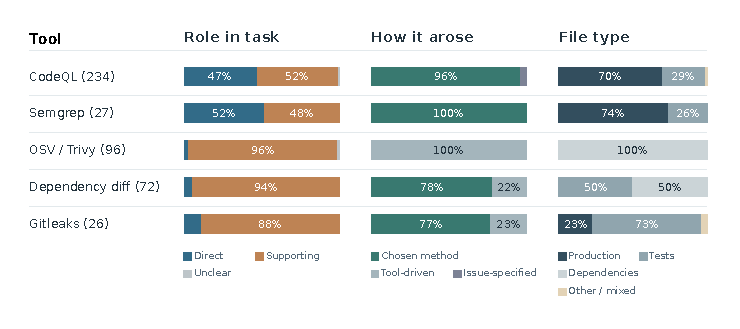
\includegraphics[width=\linewidth]{assets/figures/Fig3_Scanner.pdf}
\caption{Tool-level composition of 455 mapped changes in 191 instances. Each row uses the tool's change count as denominator, and each panel has its own legend. Task-role colours denote Direct, Supporting and Unclear. The other panels show the original implementation-origin and file-type labels. These change-level labels are distinct from the 342-choice classification in Table~\ref{tab:routes}, and the version behind the origin panel is uncertain. The file-type panel retains the known dot-ai README misclassification discussed in Section~\ref{sec:s3}; it is not a corrected estimate of production exposure. All original bars and percentages are restored without recalculation.}
\Description{Three original panels show task role, implementation-origin labels and file type by reporting tool, with separate complete legends. The original values are preserved; the caption identifies the historical classification limits and the known README file-type error.}
\label{fig:scanner}
\end{figure}

\begin{table}[H]
\caption{How 342 implementation choices were classified using public evidence (455 responsible changes, 191 instances).}
\label{tab:routes}
\small
\begin{tabular}{@{}lrrrr@{}}
\toprule
\textbf{Version} & \textbf{H} & \textbf{T} & \textbf{M} & \textbf{U}\\
\midrule
Primary frozen classification & 6 & 103 & 233 & 0\\
Earlier classification snapshot & 5 & 103 & 234 & 0\\
\bottomrule
\end{tabular}
\par\smallskip\raggedright\footnotesize Among the 233 choices classified as selected among alternatives, 77 have a specific precursor, precedent or contract (T1--T3), 128 have contextual support alone (T4), four have no independently identified public explanation (T5), and 24 have critical evidence missing (Incomplete). These are the final model-assisted classifications. The preceding classification version differed for 43 implementation choices; it is shown to expose version sensitivity, not pooled into the primary analysis. Independent blind human agreement on these labels is unavailable. Similar aggregate totals do not imply stable individual classifications. ``Incomplete'' concerns the explanation tier, whereas U concerns the broader H/T/M classification; incomplete evidence for an earlier precedent does not automatically make that broader category unresolved. Zero U labels therefore does not establish complete certainty.
\end{table}

\suppbox{Additional patterns from archived records}{%
\renewcommand{\arraystretch}{1.12}%
\begin{tabularx}{\linewidth}{@{}L{3.2cm}Y@{}}
\texttt{js/insecure-\allowbreak temporary-\allowbreak file} & 44 responsible changes in 18 repositories; 26 are test-only Supporting changes.\\
\texttt{js/file-\allowbreak system-\allowbreak race} & 17 responsible changes in 13 repositories. One responsible change can be associated with multiple rules.\\
\textbf{Tool-generated choices} & At least one choice classified as mechanical appeared in 13/20 dependency-maintenance or compatibility/migration instances, versus 2/38 feature instances in the initial subset.\\
\end{tabularx}}

% =====================================================================
\FloatBarrier
\section{RQ2 Matching and Sensitivity}\label{sec:s5}

\suppbox{Matched-control procedure (RQ2)}{%
\renewcommand{\arraystretch}{1.12}%
\begin{tabularx}{\linewidth}{@{}L{0.8cm}Y@{}}
\textbf{01} & Identify eligible candidate controls. Same-repository candidates must cover the positive's completed checks; cross-repository candidates must have exactly the same set of completed checks.\\
\textbf{02} & Apply the frozen date and change-size calipers (Section~\ref{sec:rq2-design}); exclude ineligible candidate pairs.\\
\textbf{03} & Solve one-to-one matching without replacement, prioritising maximum pair count, then same-repository pairs, then minimum normalised date/size distance, in that order.\\
\textbf{04} & Freeze the pair map; only then join the issue-wording annotations. No pair-specific re-annotation. Figure~\ref{fig:rq2-method} shows the matching stages.\\
\end{tabularx}}

\suppbox{Issue-wording codes and inference boundary}{%
\renewcommand{\arraystretch}{1.12}%
\begin{tabularx}{\linewidth}{@{}L{2.3cm}Y@{}}
\textbf{Problem only} & Problem or goal without a proposed implementation.\\
\textbf{Suggests solution} & Approach proposed, without fixing the method.\\
\textbf{Explicit instruction} & A concrete implementation instruction; distinct from H (exact mechanism prescribed).\\
\textbf{Statistical test} & Paired $3\times3$ Stuart--Maxwell test with matched pairs as units; categories are not a numeric score. Explicit-versus-other proportions are descriptive.\\
\textbf{Multiple tests} & Holm correction covered nine comparisons. These assessed issue purpose, instruction specificity, issue--PR goal alignment, implementation category, formal human review, issue-to-PR delay, shared issue/PR authorship, prior requester activity, and coding-agent or tool identity.\\
\textbf{Interpretation} & Issue-wording specificity is not a measurement of security requirements or the precise risky mechanism.\\
\end{tabularx}}

\begin{figure}[H]
\centering
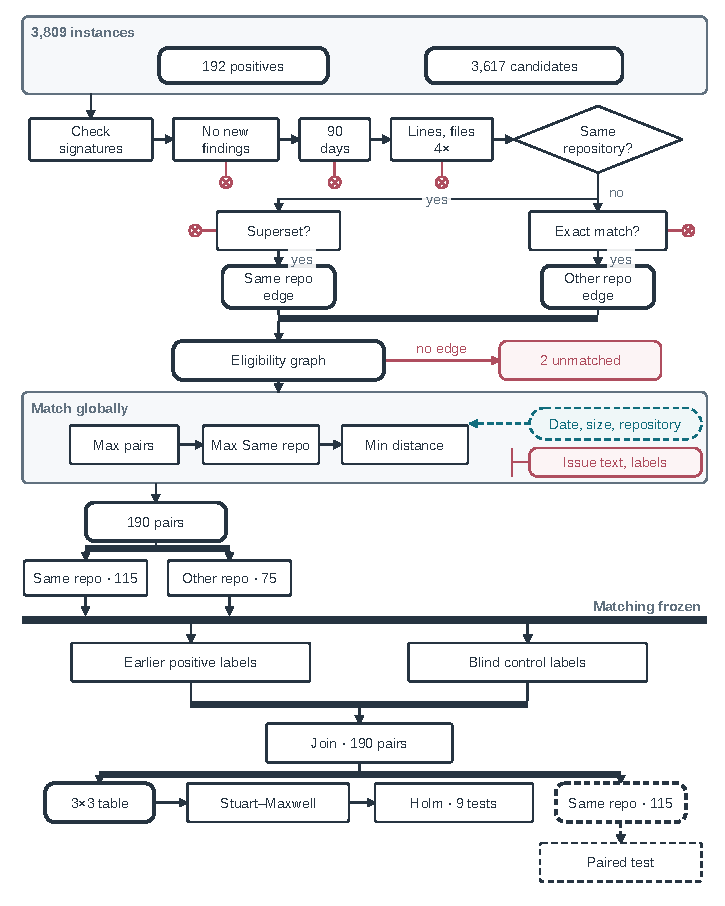
\includegraphics[width=0.85\textwidth]{assets/figures/RQ2_Methodology.pdf}
\caption{RQ2 matched comparison, showing eligibility checks and one-to-one matching. Labels were joined to pairs only after matching was frozen. Red end markers indicate failed eligibility checks; the dashed branch shows the nested same-repository sensitivity analysis.}
\Description{Finding-positive instances and candidate controls are filtered by completed checks, date and change size. Global matching prioritises pair count and same-repository pairs before issue labels are joined.}
\label{fig:rq2-method}
\end{figure}

\begin{table}[H]
\caption{RQ2 matching diagnostics, subsets and secondary comparisons. Values come from archived analysis unless identified as recomputed.}
\label{tab:rq2-diag}
\footnotesize\renewcommand{\arraystretch}{1.12}
\begin{tabularx}{\linewidth}{@{}L{5.0cm}Y@{}}
\toprule
\textbf{Quantity} & \textbf{Value}\\
\midrule
\multicolumn{2}{@{}l}{\textit{Matching}}\\
Positives matched & 190 of 192 (115 same-repository, 75 cross-repository); two without an eligible control\\
Calipers & 90 days PR date; about fourfold changed lines and files\\
Median absolute date separation & 6.66 days\\
Median larger-to-smaller ratio & 1.26 changed lines; 1.22 changed files\\
\multicolumn{2}{@{}l}{\textit{Wording, all 190 pairs (Table~\ref{tab:rq2})}}\\
Explicit instruction & 121 positives vs 148 controls ($-14.2$ points)\\
Discordant pairs & Explicit 23 positive-only vs 50 control-only; Suggests solution 33 vs 9; Problem only 26 vs 23 (recomputed from Table~\ref{tab:rq2})\\
\multicolumn{2}{@{}l}{\textit{Subsets (nested, not independent)}}\\
Original-cohort pairs & 73 of 121 vs 93 of 121 explicit ($-16.5$ points)\\
Same-repository pairs & 77 of 115 vs 95 of 115 explicit; paired $p=0.00645$\\
Direct-only positive instances & 48 of 78 vs 58 of 78 explicit\\
Supporting-only positive instances & 60 of 94 vs 75 of 94 explicit\\
Mixed positive instances & 13 of 15 on both sides; three pairs unassigned\\
\multicolumn{2}{@{}l}{\textit{Secondary comparison}}\\
Issue--PR goal alignment & 160 of 190 vs 183 of 190; $p=0.00102$, $p_{\mathrm{Holm}}=0.00815$; within repositories $p\approx0.077$\\
\bottomrule
\end{tabularx}
\end{table}

\begin{figure}[H]
\centering
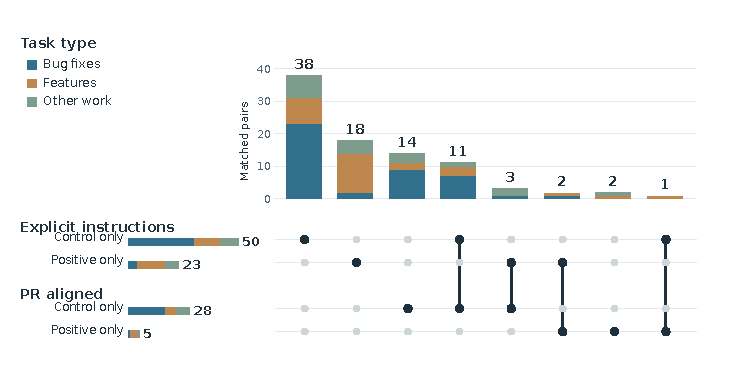
\includegraphics[width=0.85\linewidth]{assets/figures/Fig4_RQ2.pdf}
\caption{RQ2 paired differences in issue explicitness and PR goal alignment, by task type of the finding-positive issue. Bars show the 89 of 190 pairs that differ on at least one measure; the other 101 have the same status on both sides. Descriptive, not causal.}
\Description{The figure displays paired differences in explicit implementation instructions and issue to PR goal alignment for 89 discordant matched pairs, grouped by task type. The other 101 pairs have matching status on both measures.}
\label{fig:rq2-results}
\end{figure}

% =====================================================================

\FloatBarrier
\section{RQ3 Replay Evidence}\label{sec:s6}

\begin{table}[H]
\caption{Inputs for the retrospective O/W/P comparison. W and P use information from the historical warning; they do not test whether equivalent guidance could be identified prospectively.}
\label{tab:m2}
\footnotesize\renewcommand{\arraystretch}{1.12}
\begin{tabularx}{\linewidth}{@{}L{1.5cm}YY@{}}
\toprule
\textbf{Condition} & \textbf{Information supplied} & \textbf{Interpretation}\\
\midrule
\textbf{O} & Original public issue alone. & Baseline reimplementation.\\
\textbf{W} & Issue plus its historical CodeQL warning. & Retrospective warning information.\\
\textbf{P} & Issue plus a warning-derived security property, without naming the rule. & Retrospective property information.\\
\bottomrule
\end{tabularx}
\end{table}

\begin{figure}[H]
\centering
\begin{tikzpicture}[
font=\small,>={Latex[length=2mm]},
box/.style={draw=black!60,fill=black!3,rounded corners=2pt,align=center,inner sep=5pt},
wide/.style={box,text width=10.4cm},
arm/.style={box,text width=2.8cm,minimum height=1.45cm},
link/.style={->,line width=.8pt}]
\node[wide] (tasks) at (0,0) {\textbf{14 selected historical tasks}};
\node[arm] (o) at (-3.65,-1.8) {\textbf{O}\\Original issue};
\node[arm] (w) at (0,-1.8) {\textbf{W}\\Issue +\\historical warning};
\node[arm] (p) at (3.65,-1.8) {\textbf{P}\\Issue +\\warning-derived property};
\node[wide] (outputs) at (0,-3.7) {\textbf{40 retained generated patches}\\12 O, 14 W and 14 P; 12 complete triples};
\node[wide] (scans) at (0,-5.1) {Compare new CodeQL alerts against recorded baselines};
\draw[link] (tasks.south) -- (o.north);
\draw[link] (tasks.south) -- (w.north);
\draw[link] (tasks.south) -- (p.north);
\draw[link] (o.south) -- (outputs.north);
\draw[link] (w.south) -- (outputs.north);
\draw[link] (p.south) -- (outputs.north);
\draw[link] (outputs) -- (scans);
\end{tikzpicture}
\caption{The O/W/P replay comparison. Each available task-condition combination has one retained output. Independent generation sessions and functional equivalence were not verified, and missing O outputs are not counted as zero.}
\Description{Fourteen historical tasks receive original-issue, warning or property inputs. Forty outputs include twelve complete triples, whose new CodeQL alerts are compared with recorded baselines.}
\label{fig:rq3-method}
\end{figure}

\subsection*{Replay records and excluded pilot}

Section~\ref{sec:rq3-design} describes task selection and the available output-to-scan links. The syntax check covers O/W/P outputs only. The OpenAgents original-issue output (case 16633-O) recorded zero new alerts but failed that check; the check does not establish functional task completion.

A separate P1--P5 guidance pilot is excluded from these comparisons. The available records do not establish whether its summary corresponds to the intended rerun, whether the stages were independent model generations, or which pinned baseline and head scans support every result. Some outputs or intermediate records are also missing. The complete original protocol descriptions, reported counts and qualifications are preserved separately in the source package; they are not evidence of a guidance effect here.

\suppbox{Replay-case coverage}{The following six cases supplement cc-wf-studio (main text, Case~4) for the O/W/P comparison in Table~\ref{tab:replays}. Other tasks with complete triples are oh-my-claudecode \#257, opencodex \#1048, Remotion \#10147, OpenAgents \#8637 and Veritas Kanban \#906. Original-issue outputs are missing for Lepton \#226 and Trilium \#7571.}

\begin{casefile}{\textbf{Ruler symlink-safe writes}\ \ {\scriptsize\texttt{intellectronica/\allowbreak ruler}}\ \ {\scriptsize Case 3429}}{\href{https://github.com/intellectronica/ruler/issues/570}{Issue \#570}\ \ \href{https://github.com/intellectronica/ruler/pull/571}{PR \#571}\ \ \href{https://github.com/intellectronica/ruler/blob/e6eeac67de8a5afd2f00223926c156c989436482/src/agents/CrushAgent.ts}{CrushAgent.ts}}
\crow{Request}{Generated writes must not follow a symlink at the final output path, including when backups are disabled (Explicit instruction).}
\crow{Historical PR}{Replaces direct writes with \texttt{writeGeneratedFile}, which already checks for symlinks.}
\crow{Warning}{CodeQL \texttt{js/insecure-temporary-file} at \texttt{FileSystemUtils.ts}:345, a statement already in the base commit. Mapped through the flow step \texttt{CrushAgent.ts}:84 (Direct).}
\crow{Replay}{O and W each recorded one new alert; P recorded zero.}
\crow{Limit}{Zero-alert outputs are not shown to implement the task or to repair the warning site, which predates the PR.}
\end{casefile}

\begin{casefile}{\textbf{Grok CLI Telegram voice input}\ \ {\scriptsize\texttt{superagent-ai/\allowbreak grok-cli}}\ \ {\scriptsize Case 8152}}{\href{https://github.com/superagent-ai/grok-cli/issues/208}{Issue \#208}\ \ \href{https://github.com/superagent-ai/grok-cli/pull/210}{PR \#210}\ \ \href{https://github.com/superagent-ai/grok-cli/blob/80fc7fbdedacc072e9ee7eb7ac8e9a1e66d493b0/src/telegram/audio-input.ts}{audio-input.ts}}
\crow{Request}{Support voice input through Telegram (Problem only).}
\crow{Historical PR}{Fetches media from \texttt{api.telegram.org/\allowbreak file/\allowbreak bot\ldots/\allowbreak\{file\_path\}}, creates a temporary directory with \texttt{mkdtemp}, writes the downloaded audio file with mode \texttt{0600}, transcribes it, and removes the temporary directory.}
\crow{Warning}{CodeQL \texttt{js/file-access-to-http} (line 71) and \texttt{js/http-to-file-access} (line 79). Both Direct, on PR-added lines.}
\crow{Replay}{The O/W/P records contain two, one and two new alerts, respectively.}
\crow{Limit}{The reports concern network/file flows in voice processing. This is a different task from the Grok CLI file-mentions case.}
\end{casefile}

\begin{casefile}{\textbf{Open Design key storage}\ \ {\scriptsize\texttt{nexu-io/\allowbreak open-design}}\ \ {\scriptsize Case 12344}}{\href{https://github.com/nexu-io/open-design/issues/6330}{Issue \#6330}\ \ \href{https://github.com/nexu-io/open-design/pull/6356}{PR \#6356}\ \ \href{https://github.com/nexu-io/open-design/blob/b65a8b009ed95669337c8a193130a81471ecd44a/apps/daemon/src/routes/runs.ts}{runs.ts}}
\crow{Request}{Persist BYOK keys reliably on Windows and fail clearly instead of silently falling back to cloud billing (Suggests solution).}
\crow{Historical PR}{The PR rolls back the secure credential-profile design to browser-local BYOK configuration. The mapped change is a configuration-completeness check in \texttt{routes/runs.ts}:849.}
\crow{Warning}{CodeQL \texttt{js/remote-property-injection} and \texttt{js/polynomial-redos} at \texttt{byok-opencode.ts}:80 and :104, statements present before the PR. One Direct change, mapped through a flow location.}
\crow{Replay}{None of the three O/W/P outputs recorded an alert under either historical rule; their recorded alerts concern other rules.}
\crow{Limit}{Absence of the historical rules did not mean an alert-free output; the recorded alerts concern other rules.}
\end{casefile}

\begin{casefile}{\textbf{Oracle downloadable artifacts}\ \ {\scriptsize\texttt{steipete/\allowbreak oracle}}}{\href{https://github.com/steipete/oracle/issues/244}{Issue \#244}\ \ \href{https://github.com/steipete/oracle/pull/245}{PR \#245}\ \ \href{https://github.com/steipete/oracle/blob/ac32c892437ad4b92f0e1ddb5d9e90ad195e38a9/src/browser/artifacts.ts}{artifacts.ts}}
\crow{Request}{Save browser-generated downloadable artifacts rather than only linking them in a transcript.}
\crow{Historical PR}{Writes downloaded bytes using \texttt{writeBinaryBrowserArtifact}, which sanitises the filename and checks for an unused target path before writing.}
\crow{Warning}{CodeQL \texttt{js/http-to-file-access}. Extended provenance records contain a mapping, not independently revalidated for this case card; this task is outside the original 122-instance workbook.}
\crow{Replay}{The historical rule was recorded under all three O/W/P conditions.}
\crow{Limit}{Functional equivalence and any repair are not established.}
\end{casefile}

\begin{casefile}{\textbf{Neo.mjs Fleet service}\ \ {\scriptsize\texttt{neomjs/\allowbreak neo}}}{\href{https://github.com/neomjs/neo/issues/16735}{Issue \#16735}\ \ \href{https://github.com/neomjs/neo/pull/16761}{PR \#16761}\ \ \href{https://github.com/neomjs/neo/blob/6bf4ebc2d4acaea88faf293cd7e670fe9e3fd4ec/ai/scripts/diagnostics/fleetHealthcheck.mjs}{fleetHealthcheck.mjs}}
\crow{Request}{An optional authenticated Fleet server and healthcheck probe with file-sourced bearer credentials.}
\crow{Historical PR}{The probe reads a bearer token from a configured file and sends it to a configurable URL (default loopback, with a timeout).}
\crow{Warning}{CodeQL \texttt{js/file-access-to-http}, \texttt{fleetHealthcheck.mjs}:107. An extended-provenance mapping is archived but not independently revalidated here; this task is outside the original 122-instance workbook.}
\crow{Replay}{The property condition matched the original-issue condition in recorded alert counts.}
\crow{Limit}{The zero-alert W output may omit functionality. This is a different task from the Neo.mjs wake receiver.}
\end{casefile}

\begin{casefile}{\textbf{Delegate Skills Windows relay}\ \ {\scriptsize\texttt{amElnagdy/\allowbreak delegate-skills}}}{\href{https://github.com/amElnagdy/delegate-skills/issues/3}{Issue \#3}\ \ \href{https://github.com/amElnagdy/delegate-skills/pull/13}{PR \#13}\ \ \href{https://github.com/amElnagdy/delegate-skills/blob/2c8d988f0d9542f7c005d8cf7f709005a63d1ba3/skills/grok-delegate/scripts/relay.mjs}{relay.mjs}}
\crow{Request}{Fix Windows quoting and path failures in an existing codex-delegate relay.}
\crow{Historical PR}{A new Grok relay writes brief, event and result files beneath an \texttt{os.tmpdir()} path named from repository and timestamp, created recursively rather than with \texttt{mkdtemp}.}
\crow{Warning}{Four CodeQL \texttt{js/insecure-temporary-file} locations in \texttt{relay.mjs}. An extended-provenance mapping is archived but not independently revalidated here; this task is outside the original 122-instance workbook.}
\crow{Limit}{The linked issue and PR differ in scope, limiting what a reimplementation of the issue can test.}
\end{casefile}
